\documentclass[french,12pt,a4paper]{article}
\usepackage[T1]{fontenc}
\usepackage[utf8]{inputenc}
\usepackage[dvips]{graphicx}
%\usepackage[english]{babel}
\usepackage[frenchb]{babel}
\AddThinSpaceBeforeFootnotes % à insérer si on utilise \usepackage[french]{babel}
\FrenchFootnotes % à insérer si on utilise \usepackage[french]{babel}
\usepackage{amsmath,amsthm,amsfonts,amssymb}
\usepackage{mathrsfs}
\usepackage{array}
\usepackage{color}
\usepackage{float}
\usepackage{pstricks,pstricks-add,pst-plot,pst-tree}
\usepackage{enumerate}
\usepackage{textcomp}
\usepackage{lscape}
\usepackage{setspace}
\usepackage{lettrine}
\usepackage{lscape}
\usepackage{etex}
\usepackage{lmodern}
\usepackage{stmaryrd}
\usepackage{subfigure}
\usepackage{multido}
\usepackage{listings}
\usepackage{footnote}
\usepackage{appendix}
\usepackage{color}
\usepackage{listings}
\usepackage{tikz}
\usepackage{dsfont}
\usetikzlibrary{matrix}

\lstset{
  language={C++},
  numbers=left, numberstyle=\tiny, stepnumber=1, firstnumber=last,
  frameround=tttt, 
  frame=single, 
  float,
  captionpos=b,
  breaklines=true,
  sensitive=f,
  morestring=[d]",
  basicstyle=\small\ttfamily,
  keywordstyle=\bf\small,
  stringstyle=\sf
}
\usepackage{fancyhdr,lastpage}
\usepackage[twoside,left=2cm,top=2.5cm,dvips,marginparwidth=1.9cm,marginparsep=0.5cm,headheight=35pt]{geometry}
%En tete et pied de page
\usepackage{fancyhdr}
\pagestyle{fancy}
\lhead{\leftmark} 
\chead{}
\rhead{PEPS}
\lfoot{ENSIMAG 3A}
\cfoot{\textit{Equipe 7}}
\rfoot{\thepage}
\renewcommand{\headrulewidth}{0pt}  
\renewcommand{\footrulewidth}{0.4pt}
\title{Projet .NET : Gestion indicielle}
\date{October 31, 475}
\author{Guillaume Fuchs, Guillaume Pelletier, Louis Perfumo, Samuel Rosilio}
%Page de garde

\begin{document}
\begin{titlepage}
\begin{center}

\textsc{\LARGE ENSIMAG}\\[1.5cm]

\textsc{\Large Manuel utilisateur}\\[0.5cm]

% Title
 \hrule
 \hrule 

\vspace{7mm}
{ \huge \bfseries Playlist 2  }

\vspace{7mm}
\hrule
\hrule

\vspace{7mm}
% Author and supervisor
\begin{minipage}{0.4\textwidth}
\begin{flushleft} \large
\emph{Etudiants:}\\
Guillaume \textsc{Fuchs},\\
Guillaume \textsc{Pelletier},\\
Samuel \textsc{Rosilio},\\
Louis \textsc{Perfumo}
\end{flushleft}
\end{minipage}

\vfill

% Bottom of the page
{\large \today}

\end{center}
\end{titlepage}
\newpage

On constatera dans un premier temps que l'objectif de cette interface n'était pas de commencer à mettre en place l'interface finale mais de présenter au mieux les résultats attendus pour la version beta. Enfin il est actuellement toujours nécessaire d'ouvrir le projet et de le compiler ainsi que de le l'exécuter pour avoir accès à l'application après avoir préalablement linké la PNL au projet.

\section{Calcul du prix et des delta d'un call européen}

\indent Lorsque l'on déploie l'application, nous arrivons dans un premier temps sur l'onglet de simulation générale. Dans cet onglet, on peut distinguer un premier cadre, qui va nous permettre en entrant simplement le temps auquel on souhaite pricer ainsi que le nombre de date de rebalancement du calcul du sous jacent de recevoir le prix de cette option dont les paramètres sont stipulés juste au dessus, la largeur de l'intervalle de confiance à 95\% ainsi que le prix obtenu en utilisant la formule fermée associée à Black - Scholes.

\begin{center}
\begin{figure}[h!]
    \caption{Calcul pour t=0.5 et 50 rebalancements}
    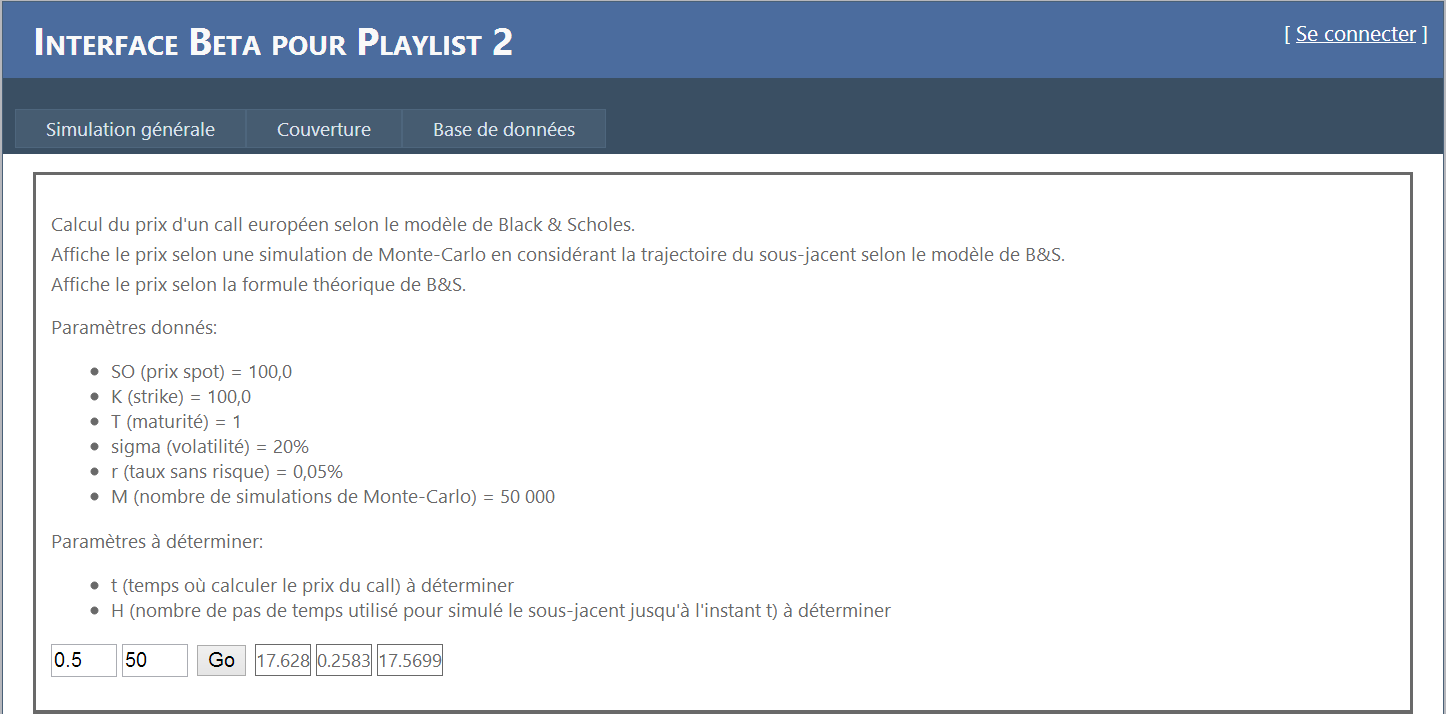
\includegraphics[scale=0.45]{../test1.png}
    \label{fig:PropProf}
\end{figure}
\end{center} 

\indent Dans un second cas, nous avons la possibilité de calculer la valeur du delta en un temps t particulier que l'on va préciser ainsi que l'intervalle de confiance associé à cette valeur et le delta théorique obtenu avec la formule fermée après avoir préciser le nombre de dates de rebalancement du sous jacent. On peut alors visualiser les différentes composantes citées précédemment pour les paramètres que nous nous sommes fixés.

\begin{center}
\begin{figure}[h!]
    \caption{Calcul pour t=0.1 et 40 rebalancements}
    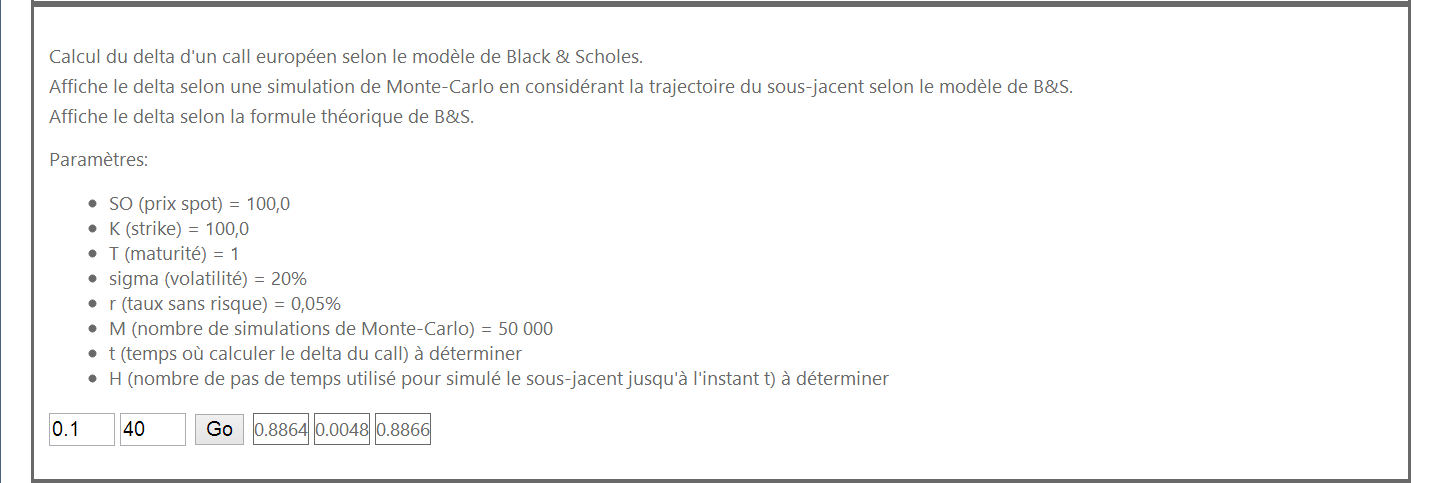
\includegraphics[scale=0.45]{../test2.png}
    \label{fig:PropProf}
\end{figure}
\end{center}



Le test permet, à partir d'un nombre \lstinline{samples} d'échantillon renseigné par l'utilisateur, de calculer la variation moyenne du prix d'un call calculé à partir de notre modèle et le prix théorique calculé grâce à la formule fermée de Black & Scholes. Lorsque l'utilisateur renseigne le champ \lstinline{samples} et appuie sur la touche \lstinline{Go}, le moteur de calcul va générer \lstinline{samples} fois une date \lstinline{t} entre 0 et 1 (1 étant la maturité de l'option) et va calculer le prix du call à cette instant là ainsi que le prix du call par la formule fermée de Black & Scholes. A la fin de la simulation, le programme va calculer la variation entre la moyenne des prix théoriques trouvés par la formule de Black & Scholes et la moyenne des prix calculés. De plus, il sera indiqué parmis les \lstinline{samples} simulations quel a été l'écart maximal trouvé pour une simulation entre le prix théorique et le prix calculé.

\begin{center}
\begin{figure}[h!]
    \caption{Calcul pour 100 échantillons}
    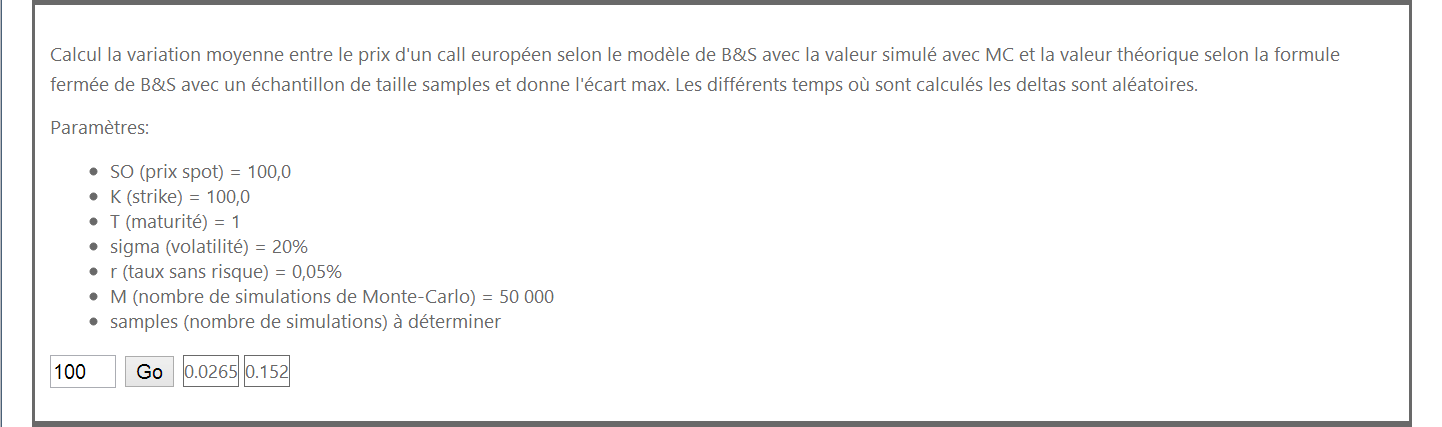
\includegraphics[scale=0.45]{../test3.png}
    \label{fig:PropProf}
\end{figure}
\end{center}

Ce test fonctionne de la même façon que le test précédent. Le prix du call est remplacé par le delta du call à différents instants entre 0 et 1.
\begin{center}
\begin{figure}[h!]
    \caption{Calcul pour 100 échantillons}
    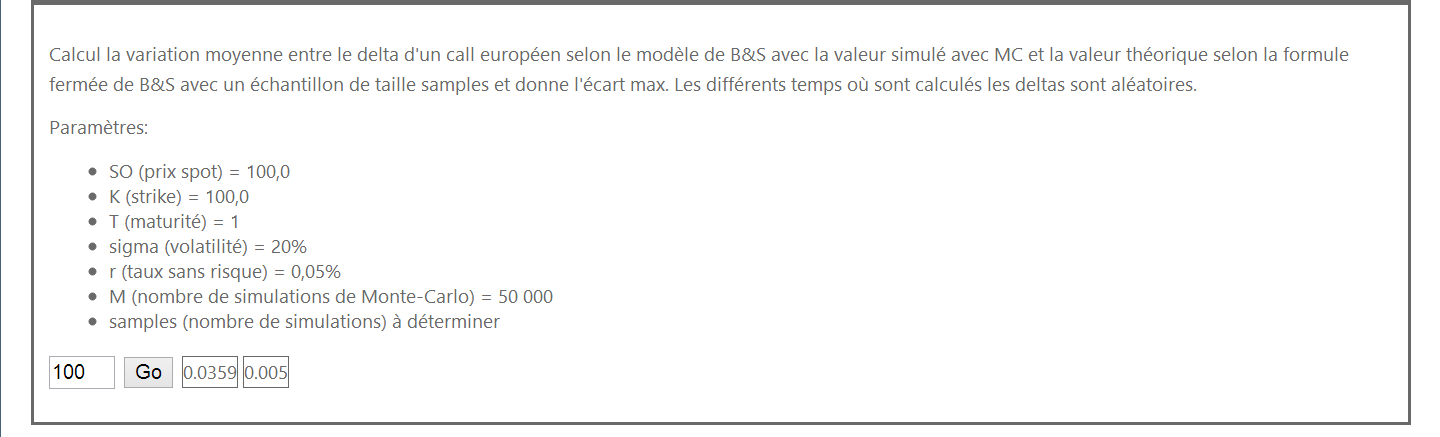
\includegraphics[scale=0.45]{../test4.png}
    \label{fig:PropProf}
\end{figure}
\end{center}


\section{Communication avec la base de données}

Dans le but de mettre en évidence la communication entre notre implémentation et la base de données, nous avons choisi de calculer les volatilités historiques de chaque actif ainsi que les correlations entre les indices pour un nombre de date données. On obtient ainsi les résultats suivants :

\begin{center}
\begin{figure}[h!]
    \caption{Exemple avec une période de 20 jours}
    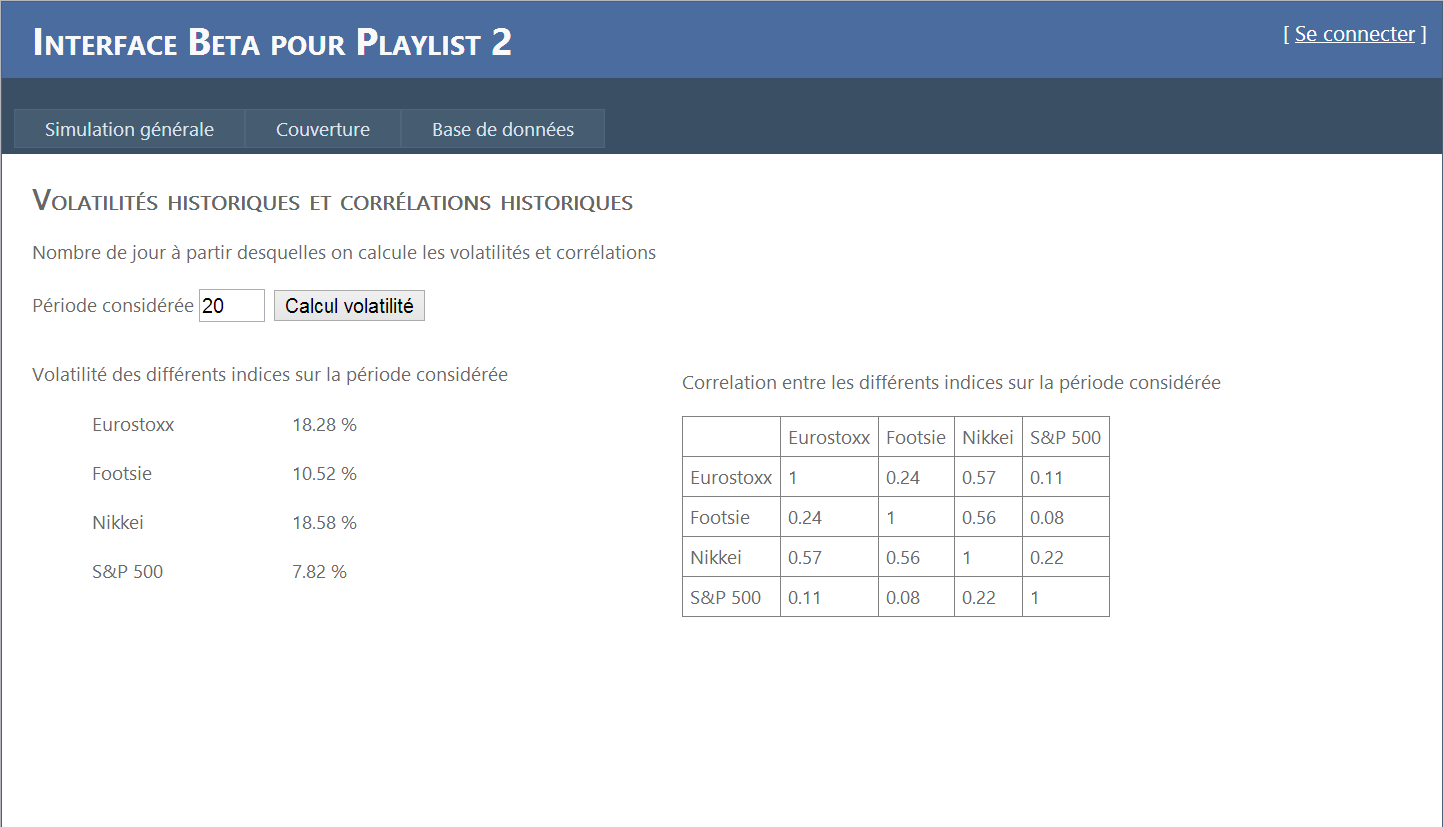
\includegraphics[scale=0.45]{Manuel2.png}
    \label{fig:PropProf}
\end{figure}
\end{center} 

On obtient alors des volatilités historiques oscillants entre 8 et 19\%. De plus les corrélations varient quant à elles entre 0.08 entre le Footsie et le S\&P $500$ et 0.57 entre le Nikkei et l'Eurostoxx.

Pour se rendre compte que les différentes valeurs exposées varient bien en fonction de la plage considérée, nous avons réalisé le même test en prenant cette fois ci une période de 60 jours, on a alors les résultats suivants :

\begin{center}
\begin{figure}[h!]
    \caption{Exemple avec une période de 60 jours}
    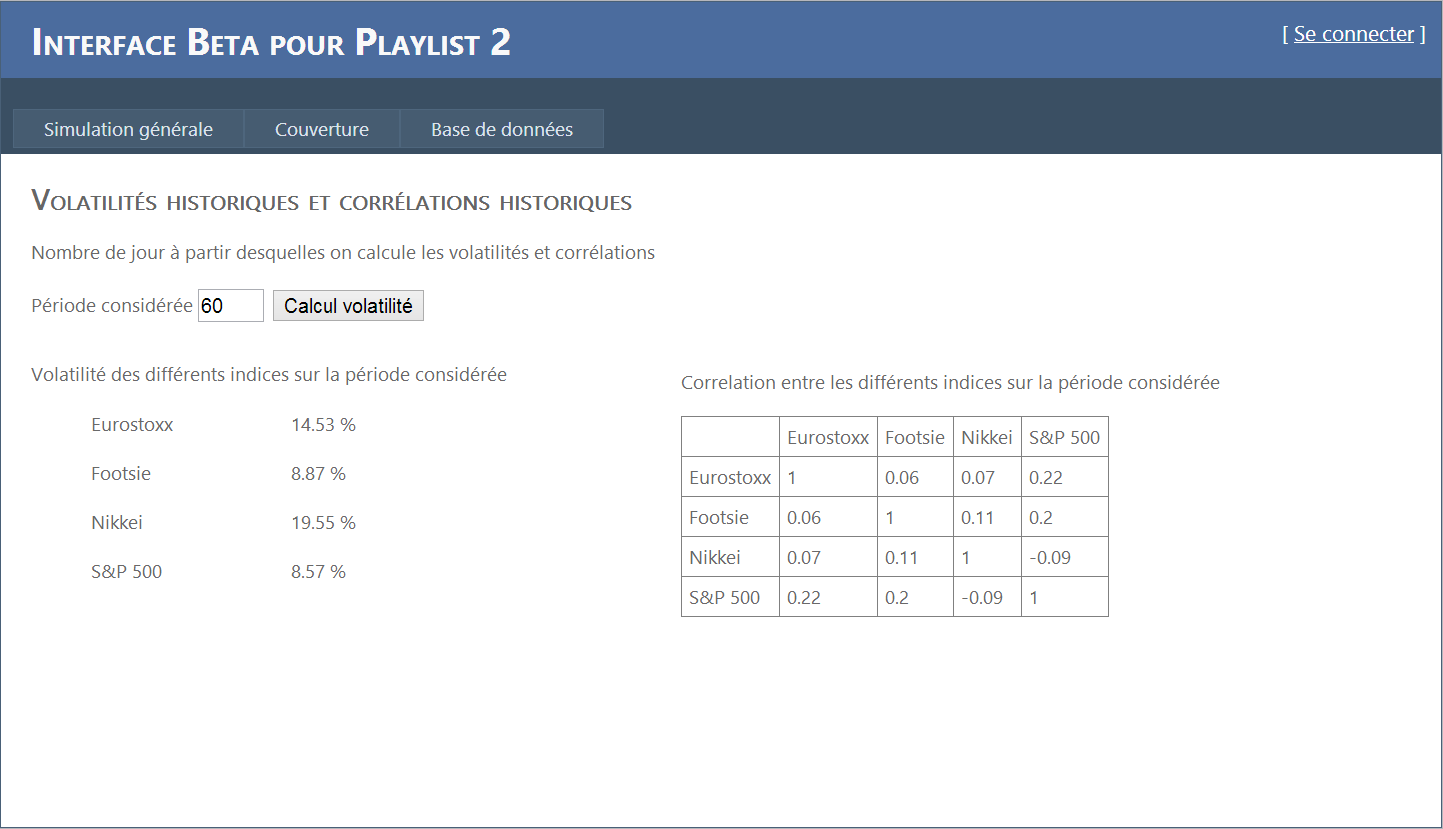
\includegraphics[scale=0.45]{Manuel1.png}
    \label{fig:PropProf}
\end{figure}
\end{center} 

Dans ce cas ci, on constate que les volatilités oscillent toujours entre 8 et 20\%. En revanche on remarque que les correlations sont très faibles sur cette période.
\newpage
\section{Calcul du portefeuille de couverture}

\indent Afin de vérifier cette fois ci au mieux l'évolution de notre portefeuille de couverture, nous proposons pour une option dont on a déjà en partie fixée les paramètres, de donner le nombre de date de rebalancement auxquelles on souhaite calculer la valeur du portefeuille de couverture.

\indent Nous avons choisi de synthétiser les différentes informations au sein d'un tableau dans lequel on peut voir les différents cours de l'action, valeurs des delta simulés, actions achetées du fait de la valeur du delta ainsi que le delta théorique et le nombre d'action a acheter associée. De plus pour un maximum de clarté, nous avons représenté l'évolution du portefeuille de couverture au cours du temps. 

\begin{center}
\begin{figure}[h!]
    \caption{Calcul pour 50 dates de rebalancements}
    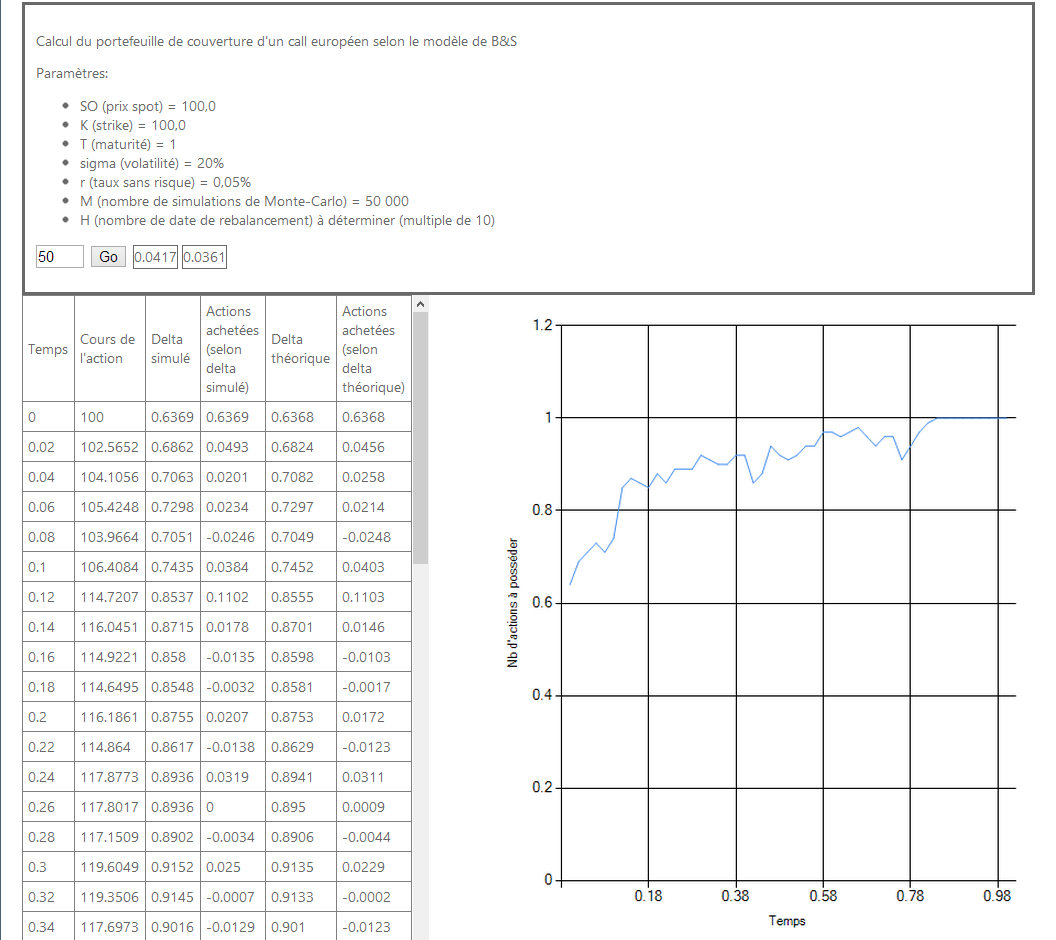
\includegraphics[scale=0.57]{../test5.png}
    \label{fig:PropProf}
\end{figure}
\end{center} 


\end{document}